\documentclass[11pt]{article}
\usepackage{fullpage}
\usepackage{amsthm}
\usepackage{amsmath} \usepackage{amssymb}
\usepackage{graphicx}

\graphicspath{ {./imgs/} }

\setlength{\parindent}{0pt}

\title{Information and Coding Theory (CO349) - Information Theory}
\author{Michael Tsang}

\newtheorem{defn}{Definition}
\newtheorem{eg}{Example}
\newtheorem{theo}{Theorem}
\newtheorem{lem}{Lemma}

\begin{document}

\maketitle

\section{Simple Codes and Coding}
\subsection{Motivation: Information and Security}
\textbf{Side-Channel Attacks:}
In optimised encryption algorithms, properties of the secret key determine the execution time.
If it is the case that zeroes lead to longer times and ones shorter then we could predict that when the algorithm runs for a longer time, the secret key contains more zeroes. \\
How much information about the secret key is revealed?
\\ \\
\textbf{Differential Privacy:}
In large statistical databases an attacker can try to reveal information (de-anonymise) individuals.
Suppose there are three individuals under 25 with hair loss registred and two individuals are getting hair loss treatment in SW7.
Kim is on the database, is 21, and lives at 170 Queen's Gate. \\
How much information about individuals is revealed?

\subsection{Entropy}
\begin{defn}
  The \textbf{entropy} of a probability distribution $p$ is:
  \[ H(p) = - \sum p(x) \log_{2} (p(x)) \].
\end{defn}

\subsection{Revision: Logarithms}
\begin{defn}
  Logarithms are defined implicitly via the equation:
  \[ x = b^{\log_{b} (x)}\]
\end{defn}

Useful identities:
\[ \log_{b} (xy) = \log_{b} (x) + \log_{b} (y) \]

\[ \log_{b} (x^{n}) = n \log_{b} (x) \]

\[ \log_{b} (x) = \frac{\log_{a} (x)}{\log_{a} (b)} \]

\subsection{Messages and Strings}
\begin{defn}
  An \textbf{alphabet} is a finite set $S$; its members $s \in S$ are \textbf{symbols}.
\end{defn}

\begin{defn}
  A \textbf{message} (or string, or word) $m$ in the alphabet $S$ is a finite sequence of elements in $S$:
  \[ m = s_1 s_2 \ldots s_n \text{ with } s_i \in S, 1 \leq i \leq n \]
  The number $n \in \mathbb{N}$ is the length of $m$, $\lvert m \rvert = n$.
\end{defn}

\begin{defn}
  A \textbf{prefix} of $m$ is defined:
  \[ m \rvert_{k} = s_1 s_2 \ldots s_k \text{ with } k \leq n \]
\end{defn}

\subsection{Notation}
\begin{defn}
  A string of length zero is denoted $\epsilon$, with $\lvert \epsilon \rvert = 0$.
\end{defn}

\begin{defn}
  $S^n$ denotes the set of all strings of length $n$, and
  \[ S^* = S^0 \cup S^1 \cup S^2 \cup \ldots \]
\end{defn}

\begin{eg}
  With the alphabet $S = \mathbb{B} = \{ 0, 1 \}$, we can produce all binary messages of a certain length $n$.
  \[ \mathbb{B}^3 = \{ 000, 001, 010, 011, 100, 101, 110, 111 \} \]
\end{eg}

\subsection{Coding}
\begin{defn}
  Let $S$ and $T$ be two alphabets; a \textbf{code} $c$ is an injective function
  \[ c : S \rightarrow T^* \]
\end{defn}

\begin{defn}
  For each symbol $s \in S$, the string $ c(s) \in T^*$ is called the \textbf{codeword} for $s$; the set of all code words is also referred to as the \textbf{code}:
  \[ C = \{ c(s) \mid s \in S \} \]
\end{defn}

An example is Morse code:
\[ c : \{ A, \ldots, Z \} \rightarrow \{ \bullet, -,\odot \} \]

\subsection{Decoding}
\begin{defn}
  A code $c : S \rightarrow T^*$ is extended to $S^*$ as follows: given a string $s_1 s_2 \ldots s_n$ in $S^*$ we define:
  \[ c(s_1 s_2 \ldots s_n) = c(s1) c(s2) \ldots c(s_n) \]
\end{defn}

\begin{defn}
  A code $c : S \rightarrow T^*$ is \textbf{uniquely decodeable (UD)} if the extended code function $c : S^* \rightarrow T^*$ is injective.
\end{defn}

This means that every string in $T^*$ corresponds to at most one message in $S^*$.

\subsection{Prefix-Free}
\begin{defn}
  A code $c : S \rightarrow T^*$ is \textbf{prefix-free (PF)} if there is no pair of codewords $q = c(s)$ and $q' = c(s')$ such that:
  \[ q' = qr \text{ for some non-empty word } r \in T^* \]
\end{defn}

\begin{eg}
  Let $S = \{ w, x, y, z\}$ with $c : S \rightarrow \mathbb{B}^*$ defined by:
  \begin{align*}
    w &\mapsto 10 & x &\mapsto 01 & y &\mapsto 11 & z &\mapsto 011
  \end{align*}
  The code is not PF, and it is not UD either:
  \begin{align*}
    wxwy &\mapsto 10011011 & wzz &\mapsto 10011011
  \end{align*}
\end{eg}

\subsection{PF implies UD}
\begin{defn}
  If a code $c : S \rightarrow T^*$ is prefix-free then it is uniquely decodeable.
\end{defn}

\textbf{Proof:}
Given that a code $c$ is prefix-free, let us assume that it is not uniquely decodeable.
Then there is an $x = x_1 x_2 \ldots x_m$ and a $y = y_1 y_2 \ldots y_n$ such that $c(x) = c(y)$, where $c(x) = c(x_1) c(x_2) \ldots c(x_m)$ and $c(y) = c(y_1) c(y_2) \ldots c(y_n)$. \\

The prefixes must be the same $c(x) \rvert_{k} = c(y) \rvert_{k}$ for any $k$, but it might be that $\lvert c(x_1) \rvert \neq \lvert c(y_1) \rvert$.
Assume that $\lvert c(x_1) \rvert \leq \lvert c(y_1) \rvert$, and take $k = \lvert c(x_1) \rvert$ then $c(x) \rvert_{k} = c(x_1) = c(y_1) \rvert_{k}$.
Thus, $c(y_1) = c(x_1) r$ for some $r \in T^*$, this contradicts PF so it must be uniquely decodeable. \\

We repeat this to cover all of $c(x) = c(y)$.

\subsection{Strings and Codes in Trees}
If we concentrate on binary codes with $T = \mathbb{B}$, any codeword in $C$ can be seen as a finite path in a binary tree.
Moreover, the codewords in $C$ can be represented as the end-points of the corresponding paths: if a code $c$ is PF then none of its decendents can represent a codeword in $C$.

\begin{eg}
  The code $C = \{ 0, 10, 110, 111 \}$ is PF, its corresponding tree is shown in figure \ref{fig:treepath}.
  \begin{figure}[h!]
    \caption{Tree for the given code $C$.}
    \centering
    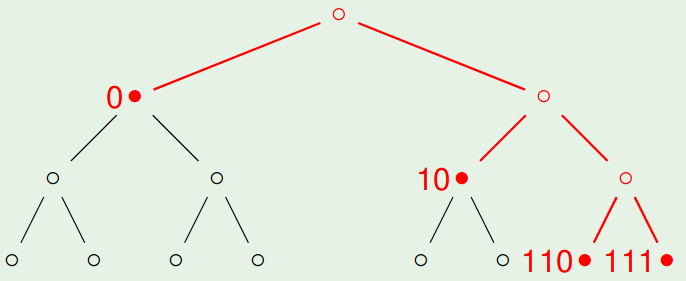
\includegraphics[width=\textwidth]{treepaths}
    \label{fig:treepath}
  \end{figure}
\end{eg}

\subsection{Parameters of a Code}
\begin{defn}
  Given a code $c: S \rightarrow T^*$, let $n_i$ denote the number of symbols $s \in S$ which are \textbf{decoded} by strings of length $i$:
  \[ n_i = \lvert \{ s \in S \mid \lvert c(s) \rvert = i \} \rvert = \lvert \{ s \in S \mid c(s) \in T^i \} \rvert \]
\end{defn}

We refer to $n_1, n_2, \ldots, n_M$ as parameters of $c$, where $M$ is the maximal length of a codeword.

\begin{defn}
  The number of all \textbf{potential codewords} of length $i$ is given by:
  \[ b^i = \lvert T^i \rvert \]
  In particular: 
  \[ b = \lvert T \rvert = b^1 \]
\end{defn}

\begin{defn}
  The \textbf{filling rate} is the fraction of possible codewords of length $i$ actually used by a code is:
  \[ \frac{n_i}{b^i} \]
\end{defn}

\subsection{Kraft-McMillan Number}
\begin{defn}
  Given a code $c : S \rightarrow T^*$ with parameters $n_1, n_2, \ldots, n_M$, the \textbf{Kraft-McMillan number} of $c$ is:
  \[ K = \sum_{i = 1}^{M} \frac{n_i}{b^i} = \frac{n_1}{b} + \frac{n_2}{b^2} + \ldots + \frac{n_M}{b^M} \]
\end{defn}

\begin{eg}
  Considering a binary code $C = \{ 0, 10, 110, 111 \}$:
  \[ K = \frac{1}{2} + \frac{1}{4} + \frac{2}{8} = \frac{8}{8} = 1 \]
\end{eg}

\subsection{Existence of PF Codes}
\begin{theo}
  Given an alphabet $T$ with $\lvert T \rvert = b$ and parameters $n_1, n_2, \ldots, n_M \in \mathbb{N}$, if $K \leq 1$ then there exists a PF $b$-ary code $c : S \rightarrow T^*$ with these parameters.
\end{theo}

That is, there is a PF $b$-ary code with $n_1$ codewords of length $1$, $n_2$ codewords of length $2$, \ldots, $n_M$ codewords of length $M$.
In fact, if $K < 1$ then there is a more optimal PF code. \\

\textbf{Proof:}
Any partial sum of the one defining $K$ also fulfills $\sum_{i} \frac{n_i}{b^i} \leq 1$.
e.g.\ $\frac{n_1}{b^1} \leq 1$, $\frac{n_2}{b^2} \leq 1$, etc.

This implies:
\begin{align*}
  n_1 &\leq b & n_2 &\leq b(b^1 - n_1) & n_3 \leq b(b^3 - n_1b^1 - n_2) & &\text{etc \ldots}
\end{align*}

or in general:
\[ n_i \leq b(b^{i - 1} - n_1b^{i - 2} - n_2b^{i - 3} - \ldots - n_{i - 1}) \]

With codeword length $1$, since $n_1 \leq b^i$, we can choose any of them, $b - n_1$ words of length 1 remain as prefixes for words of length $2, 3, \ldots$

With codeword length $2$, there are $b^2$ codewords of length 2 but $b^1n_1$ are unavailable so $b^2 - b^1n_1$ are left.
However we have $n_2 \leq b(b - n_1)$ so we can make our choices, leaving $b^2 - n_1b - n_2$ prefixes of length 2 left.

With codeword length $i$, there are always $b^{i - 1} - n_1b^{i - 2} - n_2b^{i-3} - \ldots - n_{i - 1}$ prefixes of length $i - 1$ left, and from $K \leq 1$ we have:
\[ n_i \leq b(b^{i - 1} - n_1b^{i - 2} - n_2b^{i - 3} - \ldots - n_{i - 1}) \]

That is, we can choose enough codewords $n_i$ of length $i$ and enough remain.

\subsection{Encoding Strings}
\begin{defn}
  Consider a code $c : S \rightarrow T^*$ with parameters $n_1, n_2, \ldots, n_M$.
  Let $q_r(i)$ be the number of strings of length $r$ in $S^*$ encoded in a string of length $i$ in $T^*$.
\end{defn}

\begin{eg}
  Let $n_1 = 2, n_2 = 3$, what is $q_2(i)$?

  Since $x = x_1x_2 \in S^2$, then $c(x) \in T$ has lengths $2, 3, \text{ or } 4$.
  This is because $x_1, x_2 = 1 \text{ or } 2$ from the parameters.

  For $\lvert c(x_1x_2) \rvert = 2$: then $q_2(2) = n_1 \times n_1 = 2 \times 2 = 4$.

  For $\lvert c(x_1x_2) \rvert = 3$: then $q_2(3) = n_1 \times n_2 + n_2 \times n_1 = 2 \times 3 + 3 \times 2 = 12$.

  For $\lvert c(x_1x_2) \rvert = 4$: then $q_2(4) = n_2 \times n_2 = 3 \times 3 = 9$.
\end{eg}

\subsection{Generating Functions}
Generating functions are an important tool for investigating sequences, e.g.\ enumerations of combinatorial objects.

\begin{defn}
  For a sequence of numbers $q(1), q(2), q(3), \ldots$ the \textbf{generating function} $Q(x)$ is given as a polynomial (formal power series) in the unknown variable x:
  \[
    Q(x) = q(1)x + q(2)x^2 + q(3)x^3 + \ldots 
  \]

  For a code $c : S -> T^*$, we consider for $1 \leq i \leq rM$:
  \[
    q_r(i) = \lvert \{ \lvert c(s) \rvert = i \mid \lvert s \rvert = r \} \rvert
  \]

  and the generating function: 

  \[
    Q_r(x) = q_r(1)x + q_r(2)x^2 + q_r(3)x^3 + \ldots + q_r(rM)x^{rM}
  \]
\end{defn}

\subsection{Counting Principle (CP)}
\begin{theo}
  Given a UD code $c : S \rightarrow T^*$ with $\lvert c(s) \rvert \leq M$ for all $s \in S$ with generating function $Q_r(x)$ then for all $r \geq 1$:
  \[
    Q_r(x) = Q_1(x)^r
  \]
\end{theo}

\begin{eg}
  Following the previous example where $n_1 = 2, n_2 = 3$, what is the relationship between $Q_1$ and $Q_2$?

  It is clear that $q_1(1) = n_1 = 2$ and $q_1(2) = n_2 = 3$.
  We therefore have that:
  \begin{align*}
    Q_1(x) &= 2x + 3x^2 & Q_2(x) &= 4x^2 + 12x^3 + 9x^4
  \end{align*}
  and thus can see that:
  \[
    (Q_1(x))^2 = Q_2(x)
  \]
\end{eg}

\subsection{Kraft-McMillan Number for UD Codes}
\begin{theo}
  If there exists a UD code $c : S \rightarrow T^*$ with parameters $n_1, n_2, \ldots, n_M$ then $K \leq 1$.

  \[
    \exists UD \implies K \leq 1 \implies \exists PF \text{ and } PF \implies UD
  \]
\end{theo}

Then the following are equivalent for codes $c : S \rightarrow T^*$:
\begin{itemize}
  \item There exists a UD code with parameters $n_1, n_2, \ldots, n_M$.
  \item It holds that $K \leq 1$ for parameters $n_1, n_2, \ldots, n_M$.
  \item There exists a PF code with parameters $n_1, n_2, \ldots, n_M$.
\end{itemize}

\section{Probability}
Probability theory is concerned with quantifying or measuring the chances that certain events can happen.

We consider an event space, i.e.\ a finite set $\Omega$ and a set $\mathcal{B} \subseteq \mathcal{P}(\Omega)$ of measureable sets in $\Omega$ which form a Boolean algebra.
For finite sets we can use the power set $\mathcal{B} = \mathcal{P}(\Omega)$.

Probabilities are assigned via a \textbf{measure}, i.e.\ a function $Pr : \mathcal{B} \rightarrow \mathbb{R}$ or $m : \mathcal{B} \rightarrow \mathbb{R}$.

\subsection{Finite Probability Spaces}
Consider finite measureable spaces $(\Omega, \mathcal{B})$ with $\lvert \Omega \rvert = n$.

\begin{defn}
  A probability measure $Pr : \mathcal{B}$ on $(\Omega, \mathcal{B})$ has to fulfil:
  \begin{itemize}
    \item $Pr(\Omega) = 1$.
    \item $0 \leq Pr(A) \leq 1$ for all $A \in \mathcal{B}$.
    \item $Pr(A \cup B) = Pr(A) + Pr(B)$ for $A \cap B = \emptyset$.
  \end{itemize}
\end{defn}

Some further rules:
\begin{itemize}
  \item $Pr(\emptyset) = 0$.
  \item $Pr(\overline{A}) = 1 - Pr(A)$.
  \item $Pr(A \cup B) = Pr(A) + Pr(B) - Pr(A \cap B)$.
\end{itemize}

\subsection{Random Distributions}
For finite measureable spaces $(\Omega, \mathcal{B}, Pr)$ with $\lvert \Omega \rvert = n$, we can define a probability measure via atoms in $\omega \in \Omega$.

\begin{defn}
  A probability distribution is a function $\textbf{p} : \Omega \rightarrow [0, 1]$, with:
  \[
    \sum_{\omega \in \Omega} \textbf{p}(\omega) = 1
  \]
\end{defn}

If we enumerate the elements in $\Omega = \{\omega_1, \omega_2, \ldots, \omega_n \}$ in some arbitrary way, we can also represent $\textbf{p}$ by a row vector in $\mathbb{R}^n$:
\[
  \textbf{p} = (\textbf{p}(\omega_1), \textbf{p}(\omega_2), \ldots, \textbf{p}(\omega_n))
\]

\subsection{Random Variables} 
\[
  Pr(A) = \sum_{\omega \in A} \textbf{p}(\omega)
\]

\begin{defn}
  A \textbf{random variable} is a function $X : \omega \rightarrow \mathbb{R}$.
\end{defn}

\subsection{Moments in Probability}
\[
  \textbf{E}(X) = \sum_{\omega \in \Omega} \textbf{p}(\omega)X(\omega) = \sum_i \textbf{p}_i \textbf{X}_i = \mu_X
\]

\begin{align*}
  \textbf{E}(X + Y) &= \textbf{E(X)} + \textbf{E}(Y) & \textbf{E}(\alpha X) & \alpha \textbf{E}(X)
\end{align*}

\[
  Var(X) = \textbf{E}((X - \textbf{E}(X)))^2 = \textbf{E}(X^2) - (\textbf{E}(X))^2 = \sigma_X^2
\]

\subsection{Bayes Theorem and Independence}
Given two subsets $A$ and $B$ in a probability space $(\Omega, \mathcal{B}, Pr)$, the conditional probability of $A$ given that $B$ has happened is:

\[
  Pr_B(A) = Pr(A \mid B) = \frac{Pr(A \cup B)}{Pr(B)}
\]

Bayes Theorem states:
\[
  Pr_A(B) = \frac{Pr_B(A)Pr(B)}{Pr(A)} = \frac{Pr(A \mid B)Pr(B)}{Pr(A)} = Pr(A \mid B)
\]

$A$ and $B$ are independent if:
\[
  Pr(B) = Pr(B \mid A) = \frac{Pr(A \cup B)}{Pr(A)}
\]
or  
\[
  Pr(A \cup B) = Pr(A)Pr(B)
\]

\subsection{Products and Probability}
Given two probability spaces $(\Omega_1, Pr_1)$ and $(\Omega_2, Pr_2)$, to keep things simple use $\mathcal{B_i} = \mathcal{P}(\Omega_i)$, we can define a probability $Pr$ on the cartesian product $\Omega = \Omega_1 \times \Omega_2$ via:
\[
  Pr(\langle \omega_1, \omega_2 \rangle) = Pr_1(\omega_1)Pr_2(\omega_2)
\]

If $Pr_1$ and $Pr_2$ correspond to probability distributions $\textbf{p}_1$ and $\textbf{p}_2$, and $\textbf{p}$ to $Pr$ then $\textbf{p} = \textbf{p}_1 \otimes \textbf{p}_2$, the \textbf{tensor product}.

Not all distributions on $\Omega_1 \times \Omega_2$ are a product.

\subsection{Tensor/Kronecker Product}
Given a $n \times m$ matrix $\textbf{A}$ and a $k \times l$ matrix $\textbf{B}$:
\begin{align*}
  \textbf{A} &=
  \begin{pmatrix}
    a_{11} & \ldots & a_{1m} \\
    \dots & \ddots & \dots \\
    a_{n1} & \ldots & a_{nm}
  \end{pmatrix}
  &
  \textbf{B} &=
  \begin{pmatrix}
    b_{11} & \ldots & b_{1l} \\
    \dots & \ddots & \dots \\
    b_{k1} & \ldots & b_{kl}
  \end{pmatrix}
\end{align*}

The tensor or Kronecker product $\textbf{A} \otimes \textbf{B}$ is a $nk \times ml$ matrix:
\[
  \textbf{A} \otimes \textbf{B} = 
  \begin{pmatrix}
    a_{11}\textbf{B} & \ldots & a_{1m}\textbf{B} \\
    \dots & \ddots & \dots \\
    a_{n1}\textbf{B} & \ldots & a_{nm}\textbf{B}
  \end{pmatrix}
\]

Special cases are square matrices and vectors.

\subsection{Correlation}
\[
  Cov(X, Y) = \textbf{E}(X - \textbf{E}(X))\textbf{E}(Y - \textbf{E}(Y)) = \textbf{E}(XY) - \textbf{E}(X)\textbf{E}(Y)
\]

The correlation coefficient is:
\[
  \rho(X, Y) = \frac{Cov(X, Y)}{\sigma_X \sigma_Y}
\]

For independent random variables $X$ and $Y$:
\[
  \textbf{E}(XY) = \textbf{E}(X)\textbf{E}(Y)
\]
\[
  Cov(X, Y) = \rho(X, Y) = 0
\]

Note that $\rho(X, Y) = 0$ does not imply independence.

\section{Representation of Information}
Information resolves or allows us to resolve uncertainty.
The larger the resolved uncertainty, the more information we have.

This could be referred to as the surprise: if $p$ is the probability of an event, $\frac{1}{p}$ is the surprise measure.

If there are two pieces of independent information, we would like that they ``add up,'' but $Pr(A \land B) = Pr(A) \times Pr(B)$.
Using the logarithm we get an additive information measure which fulfills:
\[
  \log(\frac{1}{p_1} \times \frac{1}{p_2}) = \log(\frac{1}{p_1}) + \log(\frac{1}{p_2})
\]

\subsection{Sources}
\begin{defn}
  Let $S$ be an alphabet, a \textbf{source} $(S, \textbf{p})$ with probability distributions $\textbf{p} = \textbf{p}^{(k)} = (p_1^{(k)}, p_2^{(k)}, \ldots, p_n^{(k)})$ emits a stream (sequence) $\sigma_1 \sigma_2 \sigma_3 \ldots$ of symbols with probability:
  \[
    Pr(\sigma_k = s_i) = p_i^{(k)}
  \]

Assume identitcal $\textbf{p}^{(k)} = \textbf{p}$, but not necessarily independent.
\end{defn}

\begin{defn}
  Let $S$ be an alphabet, a \textbf{memoryless source} $(S, \textbf{p})$ emits a stream (sequence) $\sigma_1 \sigma_2 \sigma_3 \ldots$ such that for all $k$ and $l$:
  \[
    Pr(\sigma_k = s_i \and \sigma_l = s_j) = Pr(\sigma_k = s_i)Pr(\sigma_l = s_j)
  \]
\end{defn}

\begin{defn}
  A \textbf{stochastic process} on a state space $S$ is a collection of $S$-valued random variables $X_i$ with $i \in \mathbb{N} \text{or} \mathbb{Z}$.
  This allows the investigation of the probability of finite paths, traces and streams.
  The probability at any moment in time depends on the past.
\end{defn}

\begin{defn}
  A \textbf{Markov Chain} is a stochastic process where the probability at one moment in time depends on the result in the last state.
\end{defn}

\subsection{Average Word Length}
Consider a source $(S, \textbf{p})$ and a code $c : S \rightarrow T^*$.
Consider the stream of symbols we obtain by encoding $\{ s_1, \ldots, s_m \}$ via $c$.

\begin{defn}
  The \textbf{average word length} $L$ of a code $c : S \rightarrow T^*$ for a source $(S, \textbf{p})$ is:
  \[
    L = p_1l_1 + p_2l_2 + \ldots + p_ml_m = \sum_{i = 1}^m p_il_i = \textbf{E}(l)
  \]
  with $l_i = \lvert c(s_i) \rvert$, the length of codewords in $T^*$ for each $s_i \in S$.
\end{defn}

We aim to keep the average ``blow up'' of a message using a code $c$ as small as possible.

\subsection{Optimal Code}
\begin{defn}
  Given a source $(S, \textbf{p})$ and an alphabet $T$, a uniquely decodeable code $c : S \rightarrow T^*$ is optimal if there is no other code $c' : S \rightarrow T^*$ with smaller average word length.
\end{defn}

We can formulate this as an optimisation problem:
Given $b \in \mathbb{N}$ and $p_1, p_2, \ldots, p_m \in [0, 1]$ with $\sum_{i_1}^m p_i = 1$; find (positive) integers $y_1, y_2, \ldots, y_m$ such that
\begin{align*}
  \text{minimise } L &= \sum_{i = 1}^m p_iy_i & \text{subject to } K &= \sum_{i = 1}^m \frac{1}{b^{y_1}} \leq 1
\end{align*}
where we use $y_i = \lvert c(s_i) \rvert = l_i$ to express $K$ (with $m = \lvert S \rvert)$) as:
\[
  K = \sum_{i = 1}^M \frac{n_i}{b^i} = \sum_{i = 1}^M (\sum_{j = 1}^{n_i} \frac{1}{b^i}) = \sum_{i = 1}^m \frac{1}{b^{y_i}}
\]

\subsection{Entropy of a Distribution}
\begin{defn}
  Given a distribution $\textbf{p} = (p_1, p_2, \ldots, p_m)$, the entropy of \textbf{p} to base $b$ is:
  \[
    \textbf{H}_b(\textbf{p}) = \sum_{i = 1}^m p_i\log_b \frac{1}{p_i}
  \]
\end{defn}

For $p_i = 0$, we set $p_i \log_b (\frac{1}{p_i})$.

\subsection{Properties of Entropy}
For source $(\mathcal{B}, (p, 1 - p))$, the binary entropy is given by:
\[
  \textbf{h}(p) = p \cdot \log_b (\frac{1}{p}) + (1 - p) \cdot \log_b (\frac{1}{(1 - p)})
\]

We have $\textbf{h}(0) = 0 = \textbf{h}(1)$ and maximal for $\textbf{h}(\frac{1}{2}) = 1$.

We can change the base by:
\[
  \textbf{H}_a(\textbf{p}) = \log_a(b) \textbf{H}_b(\textbf{p})
\]

Except for base, entropy is uniquely defined if we require a continuous function with:
\begin{itemize}
  \item $\textbf{H}(\textbf{p})$ is maximal for uniform distribution $\textbf{p}$.
  \item $\textbf{H}(\textbf{p} \otimes \textbf{q}) = \textbf{H}(\textbf{p}) + \textbf{H}(\textbf{q} \mid \textbf{p})$.
  \item $\textbf{H}((p_1, p_2, \ldots, p_n, 0)) = \textbf{H}((p_1, p_2, \ldots, p_n))$.
\end{itemize}

with conditional entropy $\textbf{H}(\textbf{p} \mid \textbf{q}) = \sum_jq_j \cdot \textbf{H}(\textbf{p} \mid j)$.

\subsection{Comparison Theorem}
\begin{theo}
  Given probability distributions $\textbf{p} = (p_1, p_2, \ldots, p_m)$ and $\textbf{q} = (q_1, q_2, \ldots, q_m)$, then:
  \[
    \textbf{H}_b(\textbf{p}) = \sum_{i = 1}^m p_i \cdot \log_b (\frac{1}{p_i}) \leq \sum_{i = 1}^m p_i \cdot \log_b (\frac{1}{q_i}) 
  \]
  There is equality if and only if $p_i = q_i$ for all $1 \leq i \leq m$.
\end{theo}

\begin{lem}
For all $x > 0$, we have $\ln(x) \leq x - 1$ with equality iff $x = 1$.
\end{lem}

\textbf{Proof:}
Take $b = \exp$, by previous lemma we have $\ln(\frac{q_i}{p_i}) \leq \frac{q_i}{p_i} - 1$, with equality iff $p_i = q_i$.
\begin{align*}
  \sum_{i = 1}^m p_i \cdot \ln(\frac{1}{p_i}) - \sum_{i = 1}^m p_i \cdot \ln({\frac{1}{q_i}}) &= \sum_{i = 1}^m p_i \cdot \ln(\frac{q_i}{p_i}) \\
  & \leq \sum_{i = 1}^m p_i \cdot (\frac{q_i}{p_i} - 1) = \sum_{i = 1}^m q_i - \sum_{i = 1}^m p_i = 1 - 1 = 0
\end{align*}
Equality holds iff $p_i = q_i$ for all $i$.

\subsection{Uniform Distribution}
\begin{theo}
  The entropy of a probability distribution $\textbf{p}$ on $m$ symbols is at most $\log_b(m)$, i.e.
  \[
    \textbf{H}_b(\textbf{p}) \leq \log_b(m)
  \]
  There is equality iff $p_i = \frac{1}{m}$ for all symbols.
\end{theo}

\textbf{Proof:}
Given probability distributions $\textbf{p} = (p_1, p_2, \ldots, p_m)$ and take $\textbf{q} = (q_1, q_2, \ldots, q_m)$ with $q_i = \frac{1}{m}$ for all $1 \leq i \leq m$, then we have:
\[
  \textbf{H}_b(\textbf{p}) \leq \sum_{i = 1}^m p_i \cdot \log_b(m) = \log_b(m)
\]
There is equality iff $p_i = q_i = \frac{1}{m}$ for all $1 \leq i \leq m$.

\subsection{Fundamental Theorem}
\begin{theo}
  The average word length $L$ of any uniquely decodeable code $c : S \rightarrow T^*$ with $\lvert T \rvert = b$ for the source $(S, \textbf{p})$ satisfies:
  \[
    L \geq \textbf{H}_b(\textbf{p})
  \]
\end{theo}

\textbf{Proof:}
With $S = \{ s_1, s_2, \ldots, s_m \}$ denote by $y_i$ the length of the codeword $s_i \in S$, then the Kraft-McMillan number is:
\[
  K =\sum_{i = 1}^m \frac{1}{b^{y_i}} = \frac{1}{b^{y_1}} + \frac{1}{b^{y_2}} + \ldots + \frac{1}{b^{y_m}}
\]
Take probability distribution $\textbf{q} = (q_1, q_2, \ldots, q_m)$ with $q_i = \frac{1}{Kb^{y_i}}$, apply the Comparison Theorem to $p$ and $q$ so that:
\[
  \textbf{H}_b(\textbf{p}) = \sum_{i = 1}^m p_i \cdot \log_b(\frac{1}{p_i}) \leq \sum_{i = 1}^m p_i \cdot \log_b(\frac{1}{q_i})
\]
which (with the $q$ chosen) gives:
\begin{align*}
  \textbf{H}_b(\textbf{p}) & \leq \sum_{i = 1}^m p_i \cdot \log_b(Kb^{y_i}) \\
  & = \sum_{i = 1}^m p_i \cdot (\log_b(K) + y_i) \\
  & = \log_b(K) + \sum_{i = 1}^m p_i \cdot y_i \\
  & = \log_b(K) + L \leq L
\end{align*}

For a UD code $K \leq 1$, it follows that $\log_b(K) \leq 0$.

\subsection{Shannon-Fano Rule}
To get $L = \textbf{H}_b(\textbf{p})$ we would need $b^{y_i} = \frac{1}{p_i}$ for all $1 \leq i \leq m$.
\textbf{Shannon-Fano (SF) Rule:}
Select the word length $y_i$ for a symbol $s_i$ the least positve integer such that $b^{y_i} \geq \frac{1}{p_i}$.
\begin{theo}
  There exists a PF code $c : S \rightarrow T^*$ with $\lvert T \rvert = b$ for the source $(S, \textbf{p})$ which satisifies $L < \textbf{H}_b(\textbf{p}) + 1$.
\end{theo}

\textbf{Proof:}
We chose $y_i$ as the least positive integer with $b^{y_i} \geq \frac{1}{p_i}$ so we have $b^{y_i - 1} < \frac{1}{p_i}$, thus $y_i - 1 < \log_b(\frac{1}{p_i})$ or $y_i < 1 + \log_b(\frac{1}{p_i})$.
\[
  L = \sum p_iy_i < \sum p_i \cdot (1 + \log_b(\frac{1}{p_i})) = 1 + \textbf{H}_b(\textbf{p})
\]

\subsection{Optimal PF Codes}
Using SF we can obtain good but not optimal codes:
\[
  \textbf{H} \leq L_{opt} \leq L_{SF} \leq \textbf{H} + 1
\]

Consider from now on only binary codes and $\log = \log_2$.

\begin{lem}
  An optimal PF code $c : S \rightarrow \mathbb{B}^*$ for a source $(S, \textbf{p})$ has the following properties:
  \begin{itemize}
    \item if the codeword $c(s')$ is longer than $c(s)$ then $p_s \geq p_{s'}$.
    \item among the codewords of maximal length there are two of the form $w0$ and $w1$ for some $w \in \mathbb{B}^*$.
  \end{itemize}
\end{lem}

\textbf{Proof:}
\begin{itemize}
  \item We have $\lvert c(s') \rvert > \lvert c(s) \rvert$ and $p_s \geq p_{s'}$.
    Define a new code which swaps the encodings of $s$ and $s'$, $\tilde{c}(s) = c(s')$ and $\tilde{c}(s') = c(s)$.
    The difference between the average world-lengths is:
    \begin{align*}
      L(\tilde{c}) - L(c) &= (p_s \lvert \tilde{c}(s') \rvert + p_{s'} \lvert \tilde(c)(s) \rvert) - (p_s \lvert c(s) \rvert + p_{s'} \lvert c(s') \rvert) \\
      &= (p_s - p_{s'})(\lvert c(s') \rvert - \lvert c(s) \rvert) \geq 0
    \end{align*}
  \item If there are no maximal codewords of the from $w0$ and $w1$, i.e.\ either of form $w0$ or $w1$ but not both, delete the last bit and obtain a better code.
\end{itemize}

\subsection{Huffman's Rules}
\begin{itemize}
  \item \textbf{H1:}
    Given a source $(S, \textbf{p})$, let $s'$ and $s''$ be symbols with the smallest probability.
    Construct a new source $(S^*, \textbf{p}^*)$ by replacing $s'$ and $s''$ with new symbol $s^*$, with probability $p_{s^*} = p_{s'} + p_{s''}$.
  \item \textbf{H2:}
    If we are given a PF binary code $h^*$ for $(S^*, p^*)$ with $h^* : s^* \mapsto w$, then define a binary code $h$ for $(S, \textbf{p})$ with $h : s' \mapsto w0$ and $h : s'' \mapsto w1$.
\end{itemize}

We apply \textbf{H1} until we have a trivial source $(\{ s^* \}, \textbf{p}^* = (1))$.

We apply \textbf{H2} to construct a new, more concrete code by splitting a symbol $s^*$ into $s'$ and $s''$.

\begin{figure}[h]
  \caption{Applying \textbf{H1}, building the tree downwards.}
  \centering
  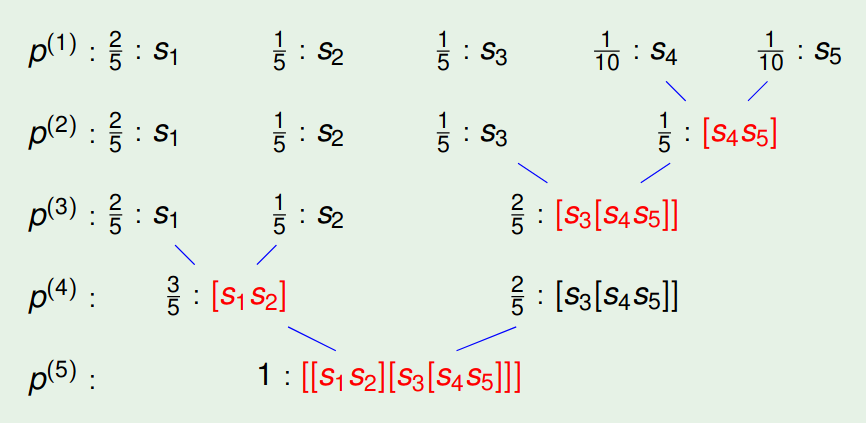
\includegraphics[width=\textwidth]{huffman1}
\end{figure}

\begin{figure}[h]
  \caption{Applying \textbf{H2}, building the tree upwards.}
  \centering
  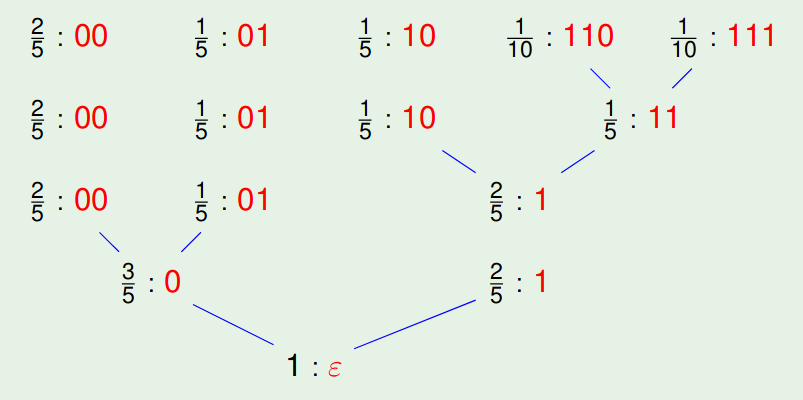
\includegraphics[width=\textwidth]{huffman2}
\end{figure}

\subsection{Quantifying the Increase in L}
\begin{lem}
  Let codes $h$ and $h^*$ be defined as required by \textbf{H2}, then the average word lengths of $h$ and $h^*$ satisfy:
  \[
    L(h) = L(h^*) + p_{s^*}^*
  \]
\end{lem}

\textbf{Proof:}
Consider $\lvert h^*(s^*) \rvert$, then $\lvert h(s') \rvert = \lvert h(s'') \rvert = \lvert h^*(s^*) \rvert + 1$, hence:
\[
  L(h) - L(h^*) = (p_{s'} + p_{s''})(\lvert h^*(s^*) \rvert + 1) - p_{s^*}^* \lvert h^*(s^*) \rvert
\]

Since $p_{s*}^* = p_{s'} + p_{s''}$, then $L(h) - L(h^*) = p_{s^*}^*$.

\subsection{Optimality of Huffman Code}
\begin{theo}
  Using Huffman's rules, if the $h^*$ is optimal for $(S^*, \textbf{p}^*)$, then $h$ is optimal for $(S, \textbf{p})$.
\end{theo}

\subsection{Coding in Blocks}
We now consider block coding, $c : S^2 \rightarrow \mathbb{B}^*, c : S^3 \rightarrow \mathbb{B}^*$, etc.
\begin{eg}
  Consider $c: \mathbb{B} \rightarrow \mathbb{B}^*$ with $\textbf{p} = (0.9, 0.1)$, it has entropy $\textbf{H}(\textbf{p}) \approx 0.469$ and $L_1 = 1$ (at best).

  Consider $c: \mathbb{B}^2 \rightarrow \mathbb{B}^*$ with $\textbf{p} = (0.81, 0.09. 0.09, 0.01)$, now $L_2 = 1.29$ or $\frac{L_2}{2} = 0.645$.

  Consider $c: \mathbb{B}^3 \rightarrow \mathbb{B}^*$ with $\textbf{p} = (0.729, 0.081, 0.081, 0.009, 0.081, 0.009, 0.009, 0.001)$, now $L_3 = 1.598$ or $\frac{L_3}{3} = 0.533$.

  We approach the theoretical minimum $\textbf{H}(\textbf{p})$.
\end{eg}

\subsection{Products and Distributions}
Consider two sets/alphabets:
\begin{align*}
  S' = \{ s'_1, s'_2, \ldots, s'_m \} & S'' = \{ s''_1, s''_2, \ldots, s''_n \}
\end{align*}
and a probability distribution $\textbf{p}$ on their cartesian product $S$:
\[
  S' \times S'' = \{ \langle s', s'' \rangle \mid s' \in S', s'' \in S'' \} = \{ s's'' \mid s' \in S', s'' \in S'' \}
\]

\begin{defn}
  Given a distribution $\textbf{p} = (p_{ij})_{i, j}$ on $S = S' \times S''$, the marginal distributions $\textbf{p}'$ on $S'$ and $\textbf{p}''$ on $S''$ are given by:
  \begin{align*}
    p'_i = \sum_{j = 1}^n p_{ij} (i = 1, \ldots, m) & p''_j = \sum_{i = 1}^m p_{ij} (j = 1, \ldots, n)
  \end{align*}
\end{defn}

$\textbf{p}'$ and $\textbf{p}''$ are independent if $p_{ij} = p'_i p''_j$ or $\textbf{p} = \textbf{p}' \otimes \textbf{p}''$.

\subsection{Entropies of Products}
\begin{theo}
  For a distribution $\textbf{p}$ on $S' \times S''$ and its marginal distributions $\textbf{p}'$ and $\textbf{p}''$, we have:
  \[
    \textbf{H}(\textbf{p}) \leq \textbf{H}(\textbf{p}') + \textbf{H}(\textbf{p}'')
  \]
  Equality holds iff $\textbf{p}'$ and $\textbf{p}''$ are independent.
\end{theo}

\textbf{Proof:}
From the right hand side:
\begin{align*}
  \textbf{H}(\textbf{p}') + \textbf{H}(\textbf{p}'') &= \sum_i p'_i \log(\frac{1}{p'_i}) + \sum_j p''_j \log(\frac{1}{p''_j}) \\
  &= \sum_i \sum_j p_{ij} \log(\frac{1}{p'_i}) + \sum_j \sum_i p_{ij} \log(\frac{1}{p''_j}) \\
  &= \sum_i \sum_j p_{ij} \log(\frac{1}{p'_ip''_j}) \\
  &= \sum_{ij} p_{ij} \log(\frac{1}{p'_ip''_j})
\end{align*}

From the left hand side:
We define a probability distribution $\textbf{q} = \textbf{p}' \otimes \textbf{p}''$ on $S' \times S''$ via $q_{ij} = p'_ip''_j$.
Applying the Comparison Theorem:
\[
  \textbf{H}(\textbf{p}) \leq \sum_{ij} p_{ij} \log(\frac{1}{q_{ij}}) = \sum_{ij} p_{ij} \log(\frac{1}{p'_ip''_j}) = \textbf{H}(\textbf{p}') + \textbf{H}(\textbf{p}'')
\]

Equality iff $\textbf{q} = \textbf{p}$, i.e.\ $\textbf{p}'$ and $\textbf{p}''$ are independent.

\subsection{Stationary Sources}
\begin{defn}
  A source emitting a stream $\sigma_1 \sigma_2 \sigma_3$ is \textbf{stationary} if, for any positive integers $l_1, l_2, \ldots, l_r$, the probabilities:
  \[
    Pr(\sigma_{k + l_1} = s_1, \sigma_{k + l_2} = s_2, \ldots, \sigma_{k + l_r} = s_r)
  \]
  depend only on the string $s_1 s_2 \ldots s_r$ and not on $k$.
\end{defn}

Typically, $l_1 = 1, l_2 = 2, \ldots, l_r = r$:
\[
  \textbf{p}^r(s_1 s_2 \ldots s_r) = Pr(\sigma_{k + l_1} = s_1, \sigma_{k + l_2} = s_2, \ldots, \sigma_{k + l_r} = s_r)
\]

We have for any stationary source that:
\[
  \textbf{p}^{r - 1}(s_1 s_2 \ldots s_{r - 1}) = \sum_{s \in S} p^r(s_1 s_2 \ldots s_{r - 1}s) = \sum_{s \in S} p^r(s s_1 s_2 \ldots s_{r - 1})
\]

A memoryless source is a stationary source with:
\[
  \textbf{p}^r(s_1 s_2 \ldots s_r) = \textbf{p}^1 (s_1) \textbf{p}^1 (s_2) \ldots \textbf{p}^1 (s_r)
\]
A stationary source which is not memoryless is one where the probability of characters appearing together in a string is different to the probability of these characters appearing independently.

\subsection{Entropy of a Stationary Source}
\begin{defn}
  The entropy $\textbf{H}$ of a stationary source with probability distribution $\textbf{p}^r$ is the infimum (greatest) over the numbers
  \begin{align*}
    \textbf{H} &= \inf \frac{\textbf{H}(\textbf{p}^r)}{r} & r &= 1, 2, 3, \ldots
  \end{align*}
\end{defn}

\begin{theo}
  For a memoryless stationary source, its entropy is $\textbf{H} = \textbf{H}(\textbf{p}^1)$.
\end{theo}

\textbf{Proof:}
For memoryless sources $\textbf{H}(\textbf{p}^2) = 2 \textbf{H}(\textbf{p}^1)$.
By induction, we have $\textbf{H}(\textbf{p}^r) = r \textbf{H}(\textbf{p}^1)$. 
Thus $\inf \frac{\textbf{H}(\textbf{p}^r)}{r} = \frac{r \textbf{H}(\textbf{p}^1)}{r} = \textbf{H}(\textbf{p}^1)$.

\subsection{Sub-Block Coding}
\begin{lem}
  Suppose $n$ is a multiple of $r$, then:
  \[
     \frac{\textbf{H}(\textbf{p}^n)}{n} \leq \frac{\textbf{H}(\textbf{p}^r)}{r}
  \]
\end{lem}

\subsection{Coding Theorem: Stationary Sources}
\begin{lem}
  For a stationary source $S$ and entropy $\textbf{H}$, given $\epsilon > 0$ there exists $n > 0$ and a PF binary code $(S^n, \textbf{p}^n)$ with $L_n$ satisfying:
  \[
    \frac{L_n}{n} < \textbf{H} + \epsilon
  \]
\end{lem}

\subsection{Algorithms for Data Compression}
We cannot use Huffman's rule for data compression as we need to know the probabilites of symbols or blocks in advance.

Data compression makes particular sense if based on blocks (not symbols), there are two approaches:
\begin{itemize}
  \item The encoding of a block is calculated in isolation: we do not consider other blocks.
  \item The codewords of a block are updated online: adaptive coding.
\end{itemize}

\subsection{Dynamic Dictionaries}
\begin{defn}
  A \textbf{dictionary} $D$ based on an alphabet $S$ is a finite sequence of distinct words in $S^*$:
  \[
    D = d_1, d_2, \ldots, d_N
  \]
  We say $i$ is the index of $d_i$.
\end{defn}

\textbf{Static Dictionary:} construct dictionary at the start and leave unchanged (Arithmetic Coding).

\textbf{Dynamic Dictionary:} update dictionary during data compression to adapt to frequency of blocks.

\subsection{Lempel, Ziv and Welch}
\begin{defn}
  Suppose we have a message $X = x_1 x_2 \ldots x_n$ in the alphabet $S = \{ s_1, s_2, \ldots, s_m \}$, and $D_0 = d_1, d_2, \ldots, d_m$ with $d_i = s_i$.
  The LZW coding rules construct $c(X) = c_1 c_2 c_3 \ldots$ as follows:
  \begin{itemize}
    \item \textbf{Step 1:} The first symbol $x_1$ (say $x_1 = s_p$) is an entry $d_p$ in $D_0$.
      Encode $x_1$ via:
      \[
        c_1 = p
      \]
      The string $x_1 x_2$ is not in $D_0$, but we define:
      \begin{align*}
        d_{m + 1} &= x_1 & D_1 &= D_0, d_{m + 1}
      \end{align*}
    \item \textbf{Step k:} ($k > 1$) We have the code $c_1 c_2 \ldots c_{k - 1}$ for the initial $x_1 x_2 \ldots x_i$ and $D_{k - 1} = d_1, d_2, \ldots, d_{m + k - 1}$.
      Find the longest string $w = x_{i + 1} \ldots x_j = d_t$ in $D_{k - 1}$.
      By definition $wx_{j + 1}$ is not in $D_{k - 1}$, encode:
      \[
        c_k = t
      \]
      and extend $D_{k - 1}$:
      \begin{align*}
        d_{m + k} &= wx_{j + 1} & D_k &= D_{k - 1}, d_{m + k}
      \end{align*}
  \end{itemize}
  Repeat until end of message $X$.
\end{defn}

\subsection{Unique Decodability for LZW}
\begin{theo}
  An LZW code constructed as above is uniquely decodable.
\end{theo}

\textbf{Proof:}
Suppose we have partially decoded $c_1 c_2 \ldots c_{k - 1}$ as $x = x_1 x_2 \ldots x_i$, and we constructed $D_{k - 1}$ by adding $k - 1$ blocks to $D_0$ with $k \geq 2$. \\

Use this to construct $c_k$ and $D_k = D_{k - 1}, d_{m + k}$.
It must be that $c_k$ is the index of a string $s_u \ldots s_v$ in $D_{k - 1}$, so the decoded string extends $x$ by $x_{i + 1} = s_u, \ldots, x_j = s_v$. \\

This leaves us to construct $D_k$ or more concretely $d_{m + k}$. \\

If $c_{k + 1} = r \leq m + k - 1$ then $d_r$ is already in $D_{k - 1}$, e.g.\ $d_r = s_a \ldots$.
Thus $x_{i + 1} = s_a$ (ignore the tail) and the new dictionary entry is $d_{m + k} = s_u \ldots s_v s_a$. \\

The other possibility is that $c_{k + 1}$ is exactly the new entry in $D_k$, i.e.\ $d_{m + k}$, or that $c_{k + 1} = m + k$.
Then $d_{m + k}$ is a string of the form $s_u \ldots s_v s_z$ with $s_z = x_{j + 1}$.
Thus $c_k c_{k + 1}$ is the encoded form of $s_u \ldots s_v s_u \ldots s_v s_z$ and in fact $x_{j + 1} = s_u$ or $d_{m + k} = s_u \ldots s_v s_u$.

We have thus reconstructed $D_k$.

\section{Transmission of Information}
\subsection{Channel}
\begin{itemize}
  \item \textbf{Code:} represents information.
  \item \textbf{Source:} produces information.
  \item \textbf{Channel:} transmits information, links sender and receiver.
\end{itemize}

\begin{figure}[h]
  \caption{Channel diagram.}
  \centering
  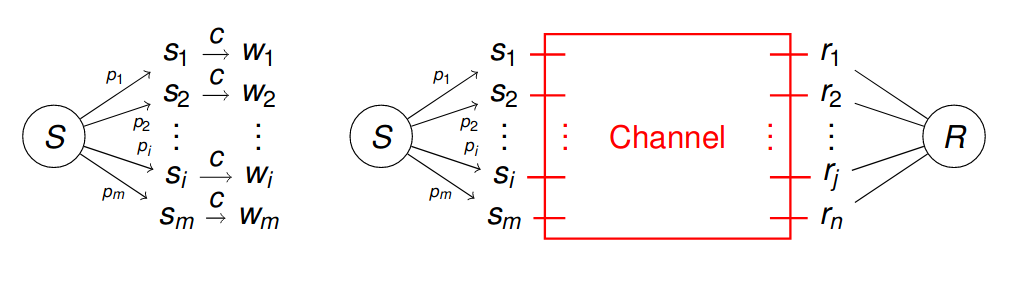
\includegraphics[width=\textwidth]{channel}
\end{figure}

\subsection{Noisy Channel}
A channel (matrix) $\Gamma$ with input set $I = \{ s_1, \ldots, s_m \}$ and output set $J = \{ r_1, \ldots, r_n \}$ is a matrix whose entries define the conditional probabilities $Pr(r_j  \mid s_i)$ with $i \in I$ and $j \in J$, i.e.
\[
  \Gamma_{ij} = Pr(j \mid i) = Pr(r_j \mid s_i)
\]

If at least one $\Gamma_{ij} \neq 0$ with $i \neq j$ then the channel is \textbf{noisy}.

In the matrix, rows correspond to inputs and columns to outputs.

\subsection{Binary Symmetric Channel}
\begin{defn}
  A \textbf{binary symmetric channel} (BSC) corresponds to the channel matrix of the form:
  \[
    \Gamma =
    \begin{pmatrix}
      \Gamma_{00} & \Gamma_{01} \\
      \Gamma_{10} & \Gamma_{11}
    \end{pmatrix}
    =
    \begin{pmatrix}
      1 - e & e \\
      e & 1- e
    \end{pmatrix}
  \]
  with error $e > 0$.
\end{defn}

\subsection{Channel Transmission}
\begin{lem}
  Each row of a channel matrix $\Gamma$ has sum $1$, i.e.\ it is \textbf{stochastic}.
  \[
    \sum_{j \in J} \Gamma_{ij} = 1 \text{ for all } i \in I
  \]
\end{lem}

\begin{theo}
  Let $\Gamma$ be a channel matrix and $(I, \textbf{p})$ and $(J, \textbf{q})$ be the sources associated to the input and output with distributions:
  \[
    \textbf{p} = (p_1, p_2, \ldots, p_m) \text{ and } \textbf{q} = (q_1, q_2, \ldots, q_n)
  \]
  then
  \[
    \textbf{q} = \textbf{p} \Gamma
  \]
\end{theo}

\textbf{Proof:}
Denote by $t_{ij}$ the probability that the input is $s_i$ and output is $r_j$, therefore $q_j = \sum_{i \in I} t_{ij}$.

In addition, $t_{ij} = Pr(\text{output} j \mid \text{input} i) \times Pr(\text{input} i) = \Gamma_{ij}p_i$.
Thus:
\[
  q_j = \sum_{i \in I} t_{ij} = \sum_{i \in I} \Gamma_{ij} p_i \text{ or } \textbf{q} = \textbf{p}\Gamma
\]

\subsection{Conditional Entropy}
Consider the probability distribution $\textbf{t}$ on $I \times J$ as
\[
  t_{ij} = Pr(\text{input $i$ and output $j$}) \neq Pr(\text{output $j$ if input $i$})
\]

We use this to construct the marginal distributions:
\begin{align*}
  p_i &= \sum_j t_{ij} & q_j &= \sum_i t_{ij} & \Gamma_{ij} &= \frac{t_{ij}}{p_i}
\end{align*}

\begin{defn}
  \textbf{Conditional entropy} $\textbf{H}(\textbf{p} \mid \textbf{q})$ (for $\textbf{q} = \textbf{p} \Gamma$) is defined as:
  \[
    \textbf{H}(\textbf{p} \mid \textbf{q}) = \textbf{H}(\textbf{t}) -  \textbf{H}(\textbf{q}) = \textbf{H}(\Gamma ; \textbf{p})
  \]

  Conditional entropy of $\textbf{p}$ with respect to transmission through $\Gamma$.
\end{defn}

\subsection{Conditional Entropy for BSC}
\begin{theo}
  Let $\Gamma$ be a BSC with a bit-error probability $e$ and source distribution $\textbf{p} = (p_0, p_1) = (p, 1 - p)$, then:
  \[
    \textbf{H}(\Gamma ; \textbf{p}) = \textbf{h}(p) + \textbf{h}(e) - \textbf{h}(q)
  \]
  where $q = p(1 - e) + (1 - p)e$ and $\textbf{h}$ is the standard entropy:
  \[
    \textbf{h}(x) = x \cdot \log_2 (\frac{1}{x}) + (1 - x) \cdot \log_2 (\frac{1}{1 - x})
  \]
\end{theo}

\textbf{Proof:}
We can compute $t_{ij} = p_i \Gamma_{ij}$:
\begin{align*}
  t_{00} &= p(1 - e) & t_{01} &= pe & t_{10} &= (1 - p)e & t_{11} &= (1 - p)(1 - e)
\end{align*}

$\textbf{t}$ can be expressed as a product of two independent distributions: $\textbf{t} = \textbf{p} \otimes \textbf{e}$.

From entropy of product of independent distributions, we get:
\[
  \textbf{H}(\Gamma ; \textbf{p}) = \textbf{H}(\textbf{t}) -  \textbf{H}(\textbf{q}) = \textbf{H}(p) + \textbf{H}(e) - \textbf{H}(q)
\]

\subsection{Channel and Source Entropy}
\begin{theo}
  Let $\Gamma$ be a channel and $\textbf{p}$ an input source distribution, then:
  \[
     \textbf{H}(\Gamma ; \textbf{p}) \leq \textbf{H}(\textbf{p}) 
  \]
  Equality holds iff $\textbf{p}$ and $\textbf{q} = \textbf{p}\Gamma$ are independent.
\end{theo}

\textbf{Proof:}
The marginal distributions of $\textbf{t}$ are $\textbf{p}$ and $\textbf{q}$, therefore $\textbf{H}(t) \leq \textbf{H}(p) + \textbf{H}(q)$.
Since $\textbf{H}(\Gamma ; \textbf{p}) = \textbf{H}(\textbf{t}) -  \textbf{H}(\textbf{q})$:
\[
  \textbf{H}(\Gamma ; \textbf{p}) + \textbf{H}(\textbf{q}) = \textbf{H}(t) \leq \textbf{H}(p) + \textbf{H}(q)
\]
or $\textbf{H}(\Gamma ; \textbf{p}) \leq \textbf{H}(\textbf{p})$.

\subsection{Capacity of a Channel}
\begin{defn}
  The \textbf{capacity} $\gamma$ of a channel $\Gamma$ is the maximum difference $\textbf{H}(\textbf{p}) - \textbf{H}(\Gamma ; \textbf{p})$ over all distributions (on $m$ elements) in $\mathcal{P}$, or:
  \[
    \gamma = \gamma(\Gamma) = \max_{\textbf{p} \in \mathcal{P}} (\textbf{H}(\textbf{p}) - \textbf{H}(\Gamma ; \textbf{p}))
  \]
\end{defn}

The maximum always exists due to the convexity of the entropy function:
\[
  \gamma(\Gamma) = \max_{\textbf{p}} (\textbf{H}(\textbf{p}) + \textbf{H}(\textbf{q}) - \textbf{H}(\textbf{t}))
\]

\subsection{BSC Capacity}

\subsection{Conditional Entropy (Redux)}

\end{document}


